The United States electrical infrastructure is complex physical structure which connects the consumers of electricity with generating assets over a large geographical area.  The nature of electricity makes the operation of this infrastructure extremely difficult and is accomplished through numerous organizations and people working together to supply electricty at the least cost while maintaining a given level of reliability.

	As of 2004, the electrical infrastructure was comprised of more than \$1 trillion in asset value.  This includes over 200,000 miles of high voltage transmission lines, 950,000 MW of generation, and 3500 utility organizations serving 283 million people.\cite{northeast_2003}  The introduction briefly looks at generation and the transmission system which efficiently moves the energy over long distances.

\subsubsection{Electricity Generation}
	Electricity is generated using a variety of fuels and procceses.  The most common method of electricity generation creates steam by heating water and which spins a turbine producing an alternating current of electricity.  The United States operates its power grid at 60 hz, that is, the direction of electrical flow switches 60 times every second.  Since the generators are tied to the grid, when the grid is stable, the generators are rotating synchronously with the power grid.  The water can be heated by different fuels such as coal, natural gas, fissioning heavy elements such as uranium, or even using geothermal temperature differentials.  The Rankine cycle is a model of converting heat into mechanical energy for steam engines.  The efficiency of the cycle is limited by the difference between the turbine entry temperature and the condenser temperature.  This means that steam cycle power plants need an external cooling source which removes the waste heat from the working fluid before it begins the cycle again.  

	The first example of a steam cycle power plant is a coal plant.  The chemical energy in coal is converted into thermal energy and byproducts such as carbon dioxide.  Power from coal provides around 40\% (for the year 2013 \cite{eia_gov}) of the electricty generation in the United States. These plants have more thermal inertia making changing the output level a slower process.  Modern coal plants achieve efficiencies of 30-40\%, that is the percentage of input energy which is injected into the grid as electricity.

	Nuclear power plants (19\% of electricity) also operate on the steam cycle, producing heat by fissioning heavy elements such as Uranium-235.  Nuclear plants have relatively slow ramping rates and cheap fuel, which lead them to be dispatched at high output rates continuously.  These plants, along with coal plants, provide the majority of baseload power production. Baseload power is the minimum amount of power that needs to be produced continuously throughout the day.  Nuclear fuel has a desirable aspect of being extremely energy dense.  The energy density of Uranium-235 is roughly 3 million times denser than coal.  This means that the waste products of this process are much less than other types of power plants and are also captured completely without being released to the environment.

	Natural gas plants (27\% of electricty) can capture, in addition to the heat energy, the combustion energy and use it to spin a gas turbine.  Gas turbines, while having a lower thermal efficiency, have the desirable trait in that you can quickly throttle production to the desired level in contrast with steam cycles.  However, by using a combination of both combustion and heat energy, combined-cycle natural gas plants can reach efficiencies of around 60\%.  These fast ramping rates and more expensive fuel lead natural gas plants to provide peaking power matching electrical demand over baseload.  Recently, with relatively cheaper natural gas and increased efficiencies from combined-cycle plants, natural gas plants are playing more of a role for electrical demand between baseload and peaking levels.    

	Hydroelectric power (6\% of electricity) has many desirable traits and it is the largest source of renewable energy generation installed around the world.  By creating a reservoir to hold a large amount of water at a high level, potential energy can be stored.  When this water is released, it becomes kinetic energy, which can be captured by a turbine and used to generate electricity.  By controlling the flow into the turbine or the amount of turbines spinning, hydro power is capable of not only storing energy, but also quickly adjusting its output rate.  However, they have the additional constraint of needing to maintain given reservoir levels throughout the year.

	In the past decade, we have introduced a sizeable amount of electricity production from renewable sources such as wind turbines and solar panels (both total 6\% of electricity, with wind comprising the majority).  These generation sources have a cheap fuel (kinetic energy from the wind and solar radiation), but are unable to control output.  

	The different characteristics of generators give them different roles to play in the operation of the power system in order to meet demand.  These various generation assets are owned by utilities, independent power producers, large industrial customers themselves, and, more recently, residential consumers.  

\subsubsection{Transmission Network}
	The production from the majority of large generation plants is at lower voltages (10kV - 25kV).  Electricity traveling in power lines lose energy due to resistive losses, which primarily goes into heating up the power line.  The resistive losses are proportional to the current.  In order to reduce losses, the voltages are stepped up to between 230 kV to 765kV for long distance transmission elements, which has the effect of reducing the current for a given amount of power.  At the demand side, there are radial tree-like distribution networks operating at low voltages (less than 1kV) which connect every demand node to the power grid.  The United States power grid is broken into three distinct power grids: Western Interconnection, Eastern Interconnection, and Texas Interconnection. Each has a network of transmission lines connecting all of the generators with all of the loads.  

	Power flows according to the laws of physics, along ``paths of least resistance", which are modeled with Kirchoff Voltage Laws (KVL) and Kirchoff Current Laws (KCL).  This means that electricity flow can't be controlled like many other complex networks such as cell phone and internet traffic, but instead follows laws of physics much like water or gas in pipe networks.  In addition, electricity flows at close to the speed of light and currently is hard to store economically, unlike water and gas.   There needs to be an instantaneous balance of generation and demand.  

\subsubsection{Organizational Structure}
The primary reliability organization which develops operating and planning standards is North American Relaibility Council (NERC) and ten regional councils. 
\begin{description}
\item[NERC] develops standards for reliable operation and planning of the bulk electric system and then monitors and assesses compliance.  Also, they provide education and training, while coordinating critical infrastructure protection, such as information exchange between reiliability service organization.  Finally, assess, analyze, and report performance and system adequacy.
\end{description}
 The primary focus of the relability and planning standards is to be able to serve all demand reliability both today and in the future.  There are 7 primary tasks:
\begin{itemize}
\item Balance power generation and demand continuously;
\item Balance reactive power supply and demand to maintain scheduled voltages;
\item Monitor flows over transmission lines and other facilities to ensure thermal limits not exceeded;
\item Keep system in stable condition;
\item Operate so that it remains in reliable condition even if contingency occurs (N-1 critiera) and when a contingency does occur, manevour to new stable N-1 position. The N-1 criteria states that the system must be robust against any single component of the power grid failing;
\item Plan, design, and maintain the system to operate reliably; and
\item Prepare for emergencies.
\end{itemize}

Within the United States, Federal Energy Regulatory Commission (FERC) is the federal agency with control over electricity sales, natural gas and oil pipelines, and hydropower projects and has increased power after the  Energy Policy Act of 2005.  This differentiates it from NERC in that it can impose mandatory standards.

\begin{description}
\item[FERC] imposes mandatory reliability standards for the bulk transmission system and imposes penalties on those that manipulate the markets.  Its primary tasks are:
\end{description}
\begin{itemize}
\item Regulate transmission and wholesale electricitity sales in interstate commerce;
\item License non-federal hydroelectric projects;
\item Ensure reliability of high voltage interstate transmission system;
\item Monitor and investigate energy markets;
\item Penalize violating entities, through civil penalties or other mean; and
\item Oversee environmental matters relating to major policy initiatives.
\end{itemize}

The restructuring of the power grid has decoupled utilities from the responsibility of maintaining a control area.  The 140 control areas are operated by the 10 regional Independent System Operators (ISOs) or Regional Transmission Organizations (RTOs).  
\begin{description}
\item[ISO/RTO] are tasked with providing least cost energy to everyone within its territory while maintaining a given level of reliability.  In order to do this, they create wholesale electricity markets in order to balance generation and load in real time at least cost.  Their tasks are:
\end{description}
\begin{itemize}
\item Manage the wholesale electricity markets while maintaining the reliability of the system; 
\item Direct the operation of the assets owned by their members; and
\item Can encompass multiple control areas within the territory that they operate.
\end{itemize}

\subsubsection{Wholesale Electricity Markets}
The ISO or RTO use 3 primary markets for determining how much each generator should produce at any given time.  The first market is bi-lateral contracts.  These are long term contracts between producers and suppliers to exchange a certain quantity of energy at a given price.  These contracts help provide reliable, long term forecasting for supply and load. This reduces exposure to the volatility of the day ahead and real time markets.  

The day ahead market takes bids from generators which contain an array of costs to produce a certain amount of electricity.  The generators also provide additional constraints which they need to operate within, such as ramping rates and start-up and shut-down times and costs.  In addition to generators information, forecasts for demand of the following day will be used to get an estimate of the amount of generation needed.  Using the transmission constraints for the given network, the ISO will clear this market during the previous day.  This process usually takes around four hours and is done with specialized optimization tools solving the optimal power flow problem with security constraints.  The outcome of this process is hourly locational marginal prices (LMP) at each location in the network for the following day.  These prices are guaranteed and any deviation from the schedule will need to be made up in the real-time market.	

The real-time market makes up for errors in forecasting as well as possible outages in generation or transmission.  This market operates on five minute intervals and can be extremely volatile.  Similar methods are used to clear this market, although simplified due to the time constraint.  Price spikes can occur during times of peak demand and a congested grid in which the price of electricity can often become over 10-20 times as expensive.  The reverse is also possible.  During times of low demand it is possible for negative prices on the real time market.  This occurs because the generators are constrained by ramping rates and there is too much production on the grid. In figure (\ref{fig:lmpmiso}), there are negative prices across the Midwest and in particular Iowa with much higher prices in Illinois.  This LMP snapshot is taken at night when there is low demand for electricity as well as increased production from wind farms located in the Midwest.  The differences in prices suggest a transmission constraint between the Upper Midwest and Illinois.   


\begin{figure}
\centering
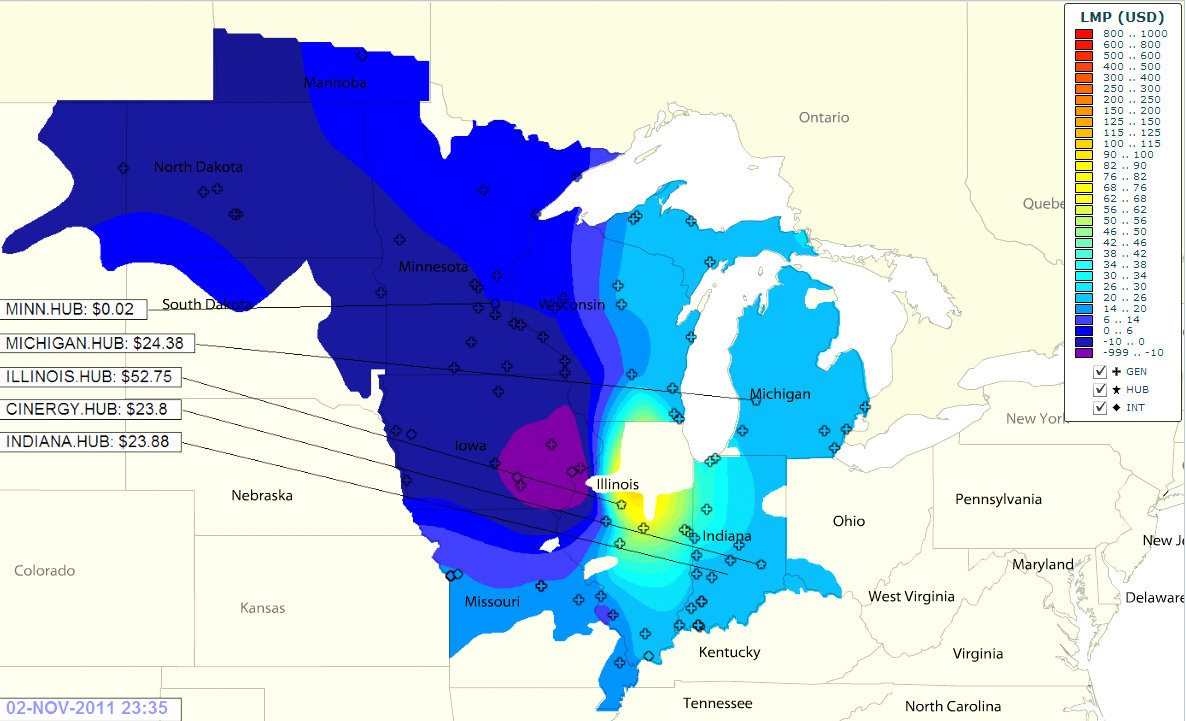
\includegraphics[width=5in]{lmp}  
\caption{Location Marginal Prices (LMP) for Midwest ISO's territory}
\label{fig:lmpmiso}
\end{figure}


\subsubsection{Operating Constraints}

In order for the power grid to operate and maintain stability, a number of things must hold.  First and foremost, there must be a continuous balance of power generation and demand.  The US grids are all operated with a target frequency of 60 hz, but the actual system frequency varies.  When there is excess generation on the grid, the frequency will increase and with a lack of generation, frequency will drop.  Since the generators are synchronized with the grid, when the frequency deviates from normal, the generators can move out of their operating limits and cause damage.  Generators will have internal protections to identify bad operating points and trip offline in order to protect themselves.  In order to protect the grid, there is automated tripping of load at certain frequency points to take customers off line and prevent total collapse.  

In addition to real power balance, reactive power supply and demand must be used to maintain scheduled voltages.  Low voltage can cause system instability and damage to motors and electrical equipment.  Also, high voltage can exceed insulation capability and cause dangerous arcs.  Reactive power is supplied through capacitor banks and generator output.

In order to protect the tranmission elements, the flows over transmission lines and other facilities must be monitored to ensure thermal limits are not exceeded.  Lines are heated by electricity flow and equipment can be damaged, such as conductors sagging from stretch and expansion due to high temperatures.  These problems are affected by ambient temperature and wind conditions.  The flow sometimes is limited so the line does not sag into obstructions such as trees and telephones.

